\section{Discussion: Guarantee-Aware Baselines and Open Science}
\label{sec:discussion}

% Auto-generated from baseline_comparison.csv
\begin{table*}[t]
\centering
\scriptsize
\caption{Guarantee-Aware Storage Architecture Comparison [Estimated from documented pricing and Analytically derived]}
\label{tab:guarantee_baselines}
\begin{tabular}{p{2.6cm} p{2.2cm} p{3.2cm} p{3.6cm} r p{2.0cm}}
\toprule
System & Availability Period & Consensus Verification & Permanence Model & Cost / MiB & Evidence Type \\
\midrule
EIP-4844 Blobs (2 gwei baseline) & Temporary ($\ge$ 4,096 epochs / $\sim$18.2 days) & Direct cryptographic commitment on Ethereum L1 (BLOBHASH / KZG) & Pruned by consensus nodes after retention window; requires external archivers & \$0.0520 & measured \\
EIP-4844 Blobs (1 wei minimal fee) & Temporary ($\ge$ 4,096 epochs / $\sim$18.2 days) & Direct cryptographic commitment on Ethereum L1 (BLOBHASH / KZG) & Pruned by consensus nodes after retention window; requires external archivers & \$0.0009 & analytically derived \\
Ethereum Calldata (Pre-EIP-7623) & Historical Chain Life (Full node history) & Merkle Patricia Trie transaction receipt root committed in block header & Retained indefinitely by archive and full nodes (subject to future EIP-4444 history pruning) & \$1.44 & analytically derived \\
Ethereum Calldata (Post-EIP-7623 Floor) & Historical Chain Life (Full node history) & Merkle Patricia Trie transaction receipt root committed in block header & Retained indefinitely by archive and full nodes (subject to future EIP-4444 history pruning) & \$3.60 & analytically derived \\
Ethereum SSTORE & Perpetual (Retained in state trie of every consensus node) & Direct real-time contract execution readability and EVM consensus state root & Permanent state until explicitly modified or cleared via SLOAD/SSTORE & \$2,949.12 & analytically derived \\
InterPlanetary File System (IPFS Pinning) & Pin-Dependent (Available only while at least one node hosts the CID) & No native consensus verification; verifiable via multihash CID match & Volatile without dedicated pinning service or economic contract & \$0.0001 & estimated from documented pricing \\
Filecoin (Storage Deal) & Contract-Dependent (typically 180 to 540 days per deal cycle) & Cryptographic Proof of Replication (PoRep) and Proof of Spacetime (PoSt) & Active contract renewal required; automatic termination upon deal expiration & \$0.0000 & estimated from documented pricing \\
Arweave (Storage Endowment) & Intended Long-Term ($\sim$200 years theoretical storage endowment) & Proof of Access (PoA / SPoRA) on independent blockweave & Protocol-enforced permanent retention funded by upfront fee endowment & \$0.0050 & estimated from documented pricing \\
Amazon S3 (Standard Storage) & Account-Dependent (SLA 99.99\% availability while subscription paid) & None (Proprietary SLA; trusted corporate provider) & Deleted upon account cancellation, subscription lapse, or TOS dispute & \$0.0000 & estimated from documented pricing \\
\bottomrule
\end{tabular}
\end{table*}


\begin{figure}[t]
\centering
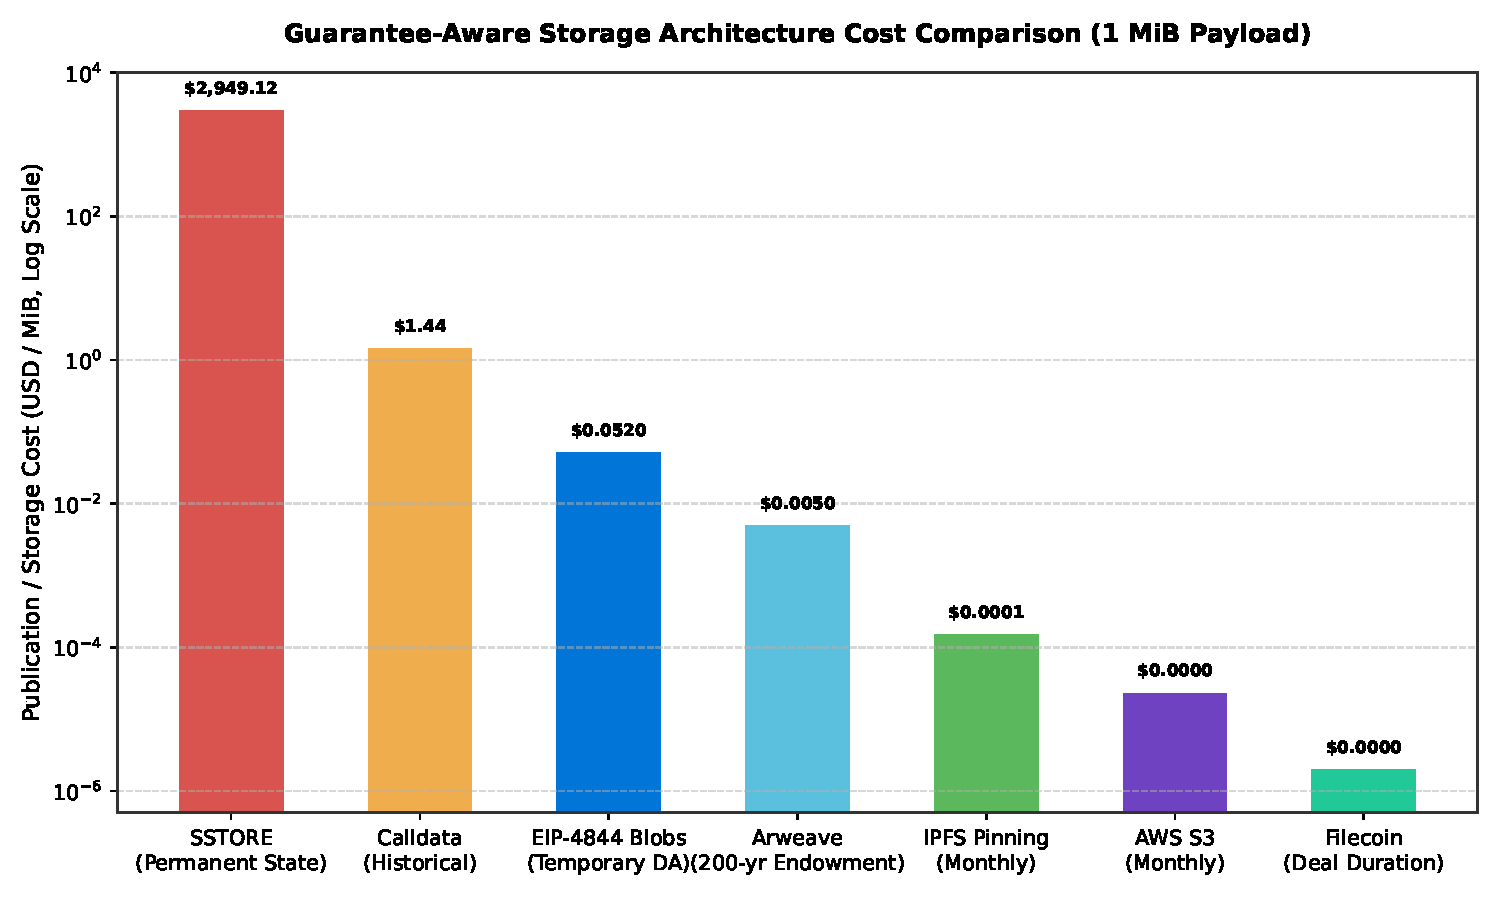
\includegraphics[width=0.95\columnwidth]{figures/fig_guarantee_cost.pdf}
\caption{Cost comparison across storage architectures under a guarantee-aware framework (log scale) [Analytical model].}
\label{fig:guarantee_cost}
\end{figure}

\subsection{Guarantee-Aware System Comparison}
Table~\ref{tab:guarantee_baselines} and Figure~\ref{fig:guarantee_cost} synthesize our guarantee-aware baseline comparison across seven decentralized and centralized storage models.

Our findings reveal why single-dimensional USD-per-gigabyte metrics fail to capture protocol trade-offs:
\begin{itemize}
    \item \textbf{EIP-4844 Blobs vs. Calldata}: Blobs provide identical Ethereum L1 consensus security at a $27.8\times$ lower publication cost. However, calldata historically persists in full node archives, whereas blobs expire after 18.2 days. Blobs are the superior choice when immediate consensus verification is required during a conference or peer-review window, provided durable external archiving is arranged.
    \item \textbf{Blobs vs. Centralized S3 / IPFS}: While commodity cloud storage is orders of magnitude cheaper in raw storage fees, it provides zero consensus anchoring. An institution can unilaterally delete an S3 bucket or alter an unversioned file without cryptographic recourse. Blobs provide an immutable, timestamped commitment anchored by the global Ethereum validator set.
\end{itemize}

\subsection{Implications for Scientific Reproducibility}
The reproducibility of computational science is challenged by the transient nature of hosted research artifacts. By coupling temporary Ethereum blob publication with verified content-addressed storage:
\begin{enumerate}
    \item \textbf{Verification During Peer Review}: Reviewers can download and verify the exact experimental trace from consensus blobs during the active review window without relying on third-party repositories.
    \item \textbf{Long-Term Citation Stability}: Persistent DOIs can point to the Ethereum dataset record and its registered CID in \texttt{ResearchArchiveRegistry.sol}, enabling future researchers to independently verify archival replicas against the immutable L1 anchor.
\end{enumerate}

We implemented and evaluated a local content-addressed archival prototype that mirrors blob payloads into a deterministic content-addressed store and verifies them against Ethereum-anchored commitments after simulated blob expiry. Public decentralized storage backends such as IPFS pinning services, Filecoin deals, and Arweave transactions were not evaluated in this study. Connecting the bridge to a public pinning or storage network remains future work, and local-store latencies are not representative of network-storage latencies.
